\documentclass[border=10pt]{standalone}
\usepackage{tikz}
\usetikzlibrary{patterns, patterns.meta}

\begin{document}
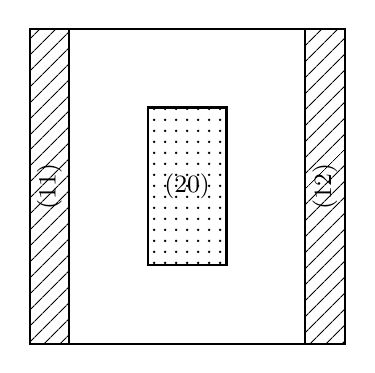
\begin{tikzpicture}
  % 외벽 (해칭)
  \fill[pattern={Lines[angle=45,distance=4pt]}] (0,0) rectangle (0.5,4);
  \fill[pattern={Lines[angle=45,distance=4pt]}] (3.5,0) rectangle (4,4);
  % 내부 공간
  \draw[thick] (0,0) rectangle (4,4);
  \draw[thick] (0.5,0) -- (0.5,4);
  \draw[thick] (3.5,0) -- (3.5,4);
  % 내부 구조물
  \fill[pattern={Dots[distance=4pt]}] (1.5,1) rectangle (2.5,3);
  \draw[thick] (1.5,1) rectangle (2.5,3);
  % 참조번호
  \node at (0.25,2) [rotate=90, font=\small] {(11)};
  \node at (3.75,2) [rotate=90, font=\small] {(12)};
  \node at (2,2)    [font=\small] {(20)};
\end{tikzpicture}
\end{document}
